\documentclass[a4paper, 12pt]{article}

\usepackage{cmap}
\usepackage{mathtext} 
\usepackage[T2A]{fontenc}
\usepackage[utf8]{inputenc}
\usepackage[english,russian]{babel}	

\usepackage{amsfonts,amssymb,amsthm,mathtools}
\usepackage{amsmath}
\usepackage{icomma} 

\usepackage{graphicx} 
\graphicspath{{Picturies/}}
\usepackage{wrapfig}

\usepackage{array,tabularx,tabulary,booktabs}
\usepackage{longtable}
\usepackage{multirow}

\usepackage{caption}
\captionsetup{labelsep=period}

\renewcommand{\phi}{\varphi}
\newcommand{\eps}{\varepsilon}
\newcommand{\parag}[1]{\paragraph*{#1:}}

\newcounter{Points}
\setcounter{Points}{1}
\newcommand{\point}{\arabic{Points}. \addtocounter{Points}{1}}

\author{Вязовкин Андрей, Б01-005} % Как меня она называет, так и надо писать
\date{5.05.21}
\title{Лабораторная работа 1.3.3. Измерение вязкости воздуха по течению в тонких трубках.}

\begin {document}

\maketitle

\parag {Цель работы} экспериментально исследовать свойства течения газов по тонким трубкам при различных числах Рейнольдса; выявить область применимости закона Пуазейля и с его помощью определить коэффициент вязкости воздуха.

\parag {В работе используются} система подачи воздуха (компрессор, поводящие трубки); газовый счетчик барабанного типа; спиртовой микроманометр с регулируемым наклоном; набор трубок различного диаметра с выходами для подсоединения микроманометра; секундомер.

\parag {Теоретическая справка} ~\\

Работа посвящена изучению течения воздуха по прямой трубе круглого сечения. Движение жидкости или газа вызывается перепадом внешнего давления на концах $\Delta P$ трубы, чему в свою очередь препятствуют силы вязкого (внутреннего) трения, действующие между соседними слоями жидкости, а также со стороны стенок трубы.

Сила вязкого трения как в жидкостях, так и в газах описывается законом Ньютона: касательное напряжение между слоями пропорционально перепаду скорости течения в направлении, поперечном к потоку. В частности, если жидкость течёт вдоль оси $x$,  а скорость течения $v_x(y)$зависит от координаты $y$, в каждом слое возникает направленное по $x$ касательное напряжение:

\[
    \tau_{xy} = - \eta \frac{\partial v_x}{\partial y}
\]

Величину $\eta$ называют коэффициентом динамической вязкости (или просто вязкостью) среды.

Объёмным расходом (или просто расходом) $Q$ называют объём жидкости,
протекающий через сечение трубы в единицу времени. Величина $Q$ зависит от
перепада давления $\Delta P$, а также от свойств газа (плотности $\rho$ и вязкости $\eta$) и от геометрических размеров (радиуса трубы $R$ и её длины $L$). Основная задача данной работы — исследовать эту зависимость экспериментально.

% Тут должен был быть анекдот про свинью. Если ваш лабник нихуя не читает и это ваша последняя работа, обязательно вставьте:
% Взяли пираты судно на абордаж, всю команду повязали, а капитану говорят, мол, показывай давай чего везешь. Ну кэп пожал плечами, говорит - пойдёмте. Спускаются вниз, а весь здоровенный трюм совершенно пуст, только одинокая свинья сидит посередине и хрюкает. Пираты охуели, ходят вокруг свиньи - ничего особенного, самая обычная, еще и воняет пиздец. Говорят капитану: - Ты ебанутый штоле? Нахуя свинью тут держишь, ее и на мясо-то посреди океана не пустишь, она жрёт только?
% Капитан плечами стоит пожимает. Пираты махнули на него рукой, повытаскивали у команды с карманов что было ценного, и отчалили.
% А капитан спустился в трюм, штаны снял, ебёт свинью и приговаривает: - Во дураки! Свинья - охуенная тема!

Характер течения в трубе может быть ламинарным либо турбулентным. 

Характер течения определяется безразмерным параметром задачи — числом Рейнольдса

\[
    Re = \frac{\rho u a}{\eta}
\]

, где $\rho$ - плотность жидкости, $u$ - скорость движения потока, $a$ - характерный размер потока.

Выпишем некоторые теоретические зависимости:

Зависимость давления в трубке от расстояния до её начала:

\[
    P(x) = P_{0} - \frac{\Delta P}{l}x
\]

Средняя скорость потока:

\[
    u = \frac{Q}{\pi R^{2}} = \frac{U_{max}}{2}
\]

Объёмный расход жидкости:

\[
    Q = \frac{\pi R^{4} \Delta P}{8\eta l}
\]

Длина трубы, через которое устанавливается пуазейлевское течение:

\[
    l_{\text{уст}} \approx 0,2R\cdot Re
\]

\parag {Экспериментальная установка} ~

\begin{figure}[!h]
    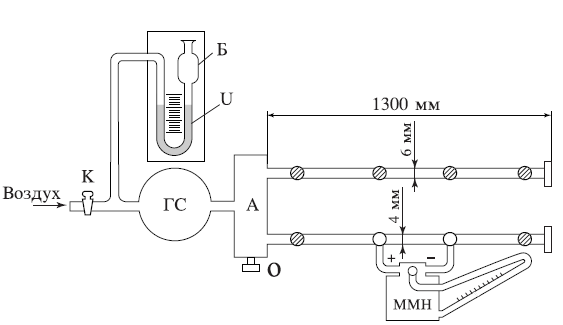
\includegraphics[scale = 0.7]{Workplace}
    \centering
    \caption{Схема установки}
\end{figure}

\parag {Ход работы} ~\\

\point Подготовим установку к работе: установим приборы по уровням, проверим наличие воды в газовом счетчике по водомерному устройству, установим на ноль мениск микроманометра. 

\point Измерим параметры окружающей среды: $t_{комн} = (23,4 \pm 0,2) ~^\circ C$, $P_{атм} = (99,6 \pm 0,5) ~кПа$, $\phi = (65 \pm 5)~\%$.

\point Запишем параметры труб:

\[
\begin {aligned}
    d_1 &= 4,10 \pm 0,05 ~мм \\
    d_2 &= 3,00 \pm 0,10 ~мм \\
    d_3 &= 5,20 \pm 0,05 ~мм 
\end {aligned}
\]

\point Рассчитаем объёмный расход $Q_{кр}$ для первой трубы, при котором наступает <<граница>> между ламинарным и турбулентным течениями. Для этого примем $Re_{кр} = 10^3$, $\eta = 2 \cdot 10^{-5} ~ Па \cdot с$.

\[
    Q_{кр} = \bar{u} \pi R_{тр}^2 = \frac{Re_{кр} ~ \eta \pi R_{тр}}{\rho} \approx 0,11 ~\frac{л}{с}
\]

\[
    где ~ \rho = \frac{p_{атм} ~\mu_{возд}}{RT} \approx 1,18 ~\frac{кг}{м^3}
\]

Найдём перепад давлений на участке $l = 50~см$:

\[
    \Delta P_{кр} = \frac{8 Q_{кр} ~\eta l}{\pi R_{тр}^4} \approx 157 Па
\]

На микроманометре это соответствует $N$ единицам шкалы:

\[
    N = \frac{\Delta P_{кр}}{9,8067 \cdot K n} \approx 76 ед.
\]

Найдём, длину трубы, через которую устанавливается пуазейлевское течение:

\[
    l_{\text{уст}} \approx 0,2 R_{тр}\cdot Re_{кр} \approx 82 см
\]

Таким образом, выбранный нами участок трубы подходит для выполнения измерений.

\point Оценим погрешности измерения объёма ($\sigma_V$) и времени ($\sigma_t$) и найдём $V_{min}$, $t_{min}$, при которых $\eps = 1\%$. Из паспорта расходометра: $\sigma_V = 0,02 дм^3 \rightarrow V_{min} = 2 дм^3$. $\sigma_t$ же найдём как среднеквадратичное отклонение времени при измерении $V_{min}$:

\begin{table}[!h]
    \begin{tabular}{|c|c|c|c|c|c|c|c|c|}
        \hline
        № измерения & 1 & 2 & 3 & 4 & 5 & 6 & 7 & 8\\ \hline
        t, c & 21.3 & 20.91 & 21.2 & 21.53 & 21.53 & 20.74 & 20.62 & 20.9 \\ \hline
    \end{tabular}
\caption{Время измерения $V_{min}$} \label{Tab:1}
\end{table}

Таким образом, $\sigma_t \approx 0,3~с \rightarrow t_{min} = 30~с$.

\point Измерим $\Delta P$, при котором становятся заметными колебания столба спирта. $\Delta P = 127$ Па. Это на $19\%$ меньше предсказанного ранее. Значит, наше предыдущее предсказание было приблизительно верным.

\point Измерим зависимость перепада  давления $\Delta P$ на  выбранном  участке трубки от расхода газа $Q$, везде берётся давление в двух последних отверстиях.

\begin{table}[!h]
\begin{longtable*}{|c|c|c|c|c|c|}
    \hline
    № & $h$, ед & $\Delta P$, Па & $V$, л & $t$, с & $Q,~\frac{л}{с}$ \\ \hline
    \endfirsthead
    \hline
    № & $h$, ед & $\Delta P$, Па & $V$, л & $t$, с & $Q,~\frac{л}{с}$ \\ \hline
    \endhead
    \hline
    \endfoot
    \hline
    \endlastfoot 
    \hline
    1 & 15 & 29.37 & 2 & 98 & 0.02 \\ \hline
    2 & 30 & 58.74 & 2 & 47.9 & 0.04 \\ \hline
    3 & 45 & 88.11 & 2 & 33.23 & 0.06 \\ \hline
    4 & 60 & 117.48 & 2.5 & 31.09 & 0.08 \\ \hline
    5 & 75 & 146.85 & 5 & 52.11 & 0.10 \\ \hline
    6 & 90 & 176.22 & 5 & 48.31 & 0.10 \\ \hline
    7 & 105 & 205.59 & 5 & 46.25 & 0.11 \\ \hline
    8 & 120 & 234.96 & 5 & 43.63 & 0.11 \\ \hline
    9 & 135 & 264.33 & 5 & 41.38 & 0.12 \\ \hline
    10 & 150 & 293.7 & 5 & 38.94 & 0.13 \\ \hline
    11 & 165 & 323.07 & 6 & 46.08 & 0.13 \\ \hline
    12 & 180 & 352.44 & 6 & 42.86 & 0.14 \\ \hline
    13 & 195 & 381.81 & 8 & 54.87 & 0.15 \\ \hline
    14 & 210 & 411.18 & 7 & 47.37 & 0.15 \\ \hline
\end{longtable*}
\caption{$Q(\Delta P)$ для первой трубы ($d = 4,1$ мм)} \label{Tab:2}
\end{table}

\begin{table}[!h]
\begin{longtable*}{|c|c|c|c|c|c|}
    \hline
    № & $h$, ед & $\Delta P$, Па & $V$, л & $t$, с & $Q,~\frac{л}{с}$ \\ \hline
    \endfirsthead
    \hline
    № & $h$, ед & $\Delta P$, Па & $V$, л & $t$, с & $Q,~\frac{л}{с}$ \\ \hline
    \endhead
    \hline
    \endfoot
    \hline
    \endlastfoot 
    \hline
    1 & 15 & 29.37 & 2 & 79.91 & 0.03 \\ \hline
    2 & 30 & 58.74 & 2.5 & 46.32 & 0.05 \\ \hline
    3 & 45 & 88.11 & 2.5 & 33.94 & 0.07 \\ \hline
    4 & 60 & 117.48 & 3 & 34.9 & 0.09 \\ \hline
    5 & 75 & 146.85 & 4 & 40.57 & 0.10 \\ \hline
    6 & 90 & 176.22 & 4 & 37.28 & 0.11 \\ \hline
    7 & 105 & 205.59 & 5 & 45.87 & 0.11 \\ \hline
    8 & 120 & 234.96 & 5 & 41.31 & 0.12 \\ \hline
    9 & 135 & 264.33 & 5 & 40.08 & 0.12 \\ \hline
    10 & 150 & 293.7 & 5 & 37.26 & 0.13 \\ \hline
    11 & 165 & 323.07 & 5 & 35.6 & 0.14 \\ \hline
    12 & 180 & 352.44 & 6 & 42.5 & 0.14 \\ \hline
    13 & 195 & 381.81 & 6 & 37.52 & 0.16 \\ \hline
    14 & 210 & 411.18 & 7 & 45.26 & 0.15 \\ \hline
\end{longtable*}
\caption{$Q(\Delta P)$ для второй трубы ($d = 3,0$ мм)} \label{Tab:3}
\end{table}

\begin{table}[!h]
\begin{longtable*}{|c|c|c|c|c|c|}
    \hline
    № & $h$, ед & $\Delta P$, Па & $V$, л & $t$, с & $Q,~\frac{л}{с}$ \\ \hline
    \endfirsthead
    \hline
    № & $h$, ед & $\Delta P$, Па & $V$, л & $t$, с & $Q,~\frac{л}{с}$ \\ \hline
    \endhead
    \hline
    \endfoot
    \hline
    \endlastfoot 
    \hline
    1 & 15 & 29.37 & 3 & 36.11 & 0.08 \\ \hline
    2 & 30 & 58.74 & 5 & 34.47 & 0.15 \\ \hline
    3 & 45 & 88.11 & 6 & 36.32 & 0.17 \\ \hline
    4 & 60 & 117.48 & 7 & 37.96 & 0.18 \\ \hline
    5 & 75 & 146.85 & 8 & 37.7 & 0.21 \\ \hline
    6 & 90 & 176.22 & 9 & 38.91 & 0.23 \\ \hline
    7 & 105 & 205.59 & 10 & 40.67 & 0.25 \\ \hline
    8 & 120 & 234.96 & 10 & 37.94 & 0.26 \\ \hline
    9 & 135 & 264.33 & 10 & 35.59 & 0.28 \\ \hline
    10 & 143 & 279.994 & 10 & 34.63 & 0.29 \\ \hline
    11 & 8 & 15.664 & 2 & 46.22 & 0.04 \\ \hline
    12 & 23 & 45.034 & 4 & 31.48 & 0.13 \\ \hline
    13 & 38 & 74.404 & 6 & 38.28 & 0.16 \\ \hline
    14 & 52 & 101.816 & 6 & 34.18 & 0.18 \\ \hline
\end{longtable*}
\caption{$Q(\Delta P)$ для третьей трубы ($d = 5,2$ мм)} \label{Tab:4}
\end{table}

\newpage

\point Измерим распределение давления газа вдоль трубки $P(x)$. Один из выходов манометра присоединим к выходу <<0>>, а другой будем перемещать по другим. Вот результаты измерений:

\begin{table}[!h]
\centering
\begin{tabular}{|c|c|c|c|c|c|c|}
    \hline
    $\Delta P$, ед & 80 & 53 & 32 & 15 \\ \hline
    $\Delta P$, Па & 156.64 & 103.774 & 62.656 & 29.37 \\ \hline
    x, см & 130.5 & 80.5 & 40.5 & 10.5 \\ \hline
\end{tabular}
\caption{Распределение давления газа вдоль трубки $P(x)$} \label{Tab:5}
\end{table}

\point Измерим зависимость расхода от радиуса трубы при заданном градиенте давления.

\begin{table}[!h]
\centering
\begin{tabular}{|c|c|c|c|c|c|c|}
    \hline
    d, мм & $\Delta P$, ед & $\Delta P$, Па & l, см & t, с & V, дм3 & Q, $\displaystyle \frac{л}{с}$ \\ \hline
    4.1 & 40 & 78.3 & 40 & 28.11 & 2 & 0.07\\ \hline
    3.0 & 30 & 58.7 & 30 & 37.11 & 2 & 0.05\\ \hline
    5.2 & 40 & 78.3 & 40 & 34.15 & 6 & 0.18\\ \hline
\end{tabular}
\caption{Расход от радиуса трубы при заданном градиенте давления} \label{Tab:6}
\end{table}

\point Построим график $Q(\Delta P)$ по таблицам \ref{Tab:2} --- \ref{Tab:4}:

\begin{figure}[!h]
    \centering
    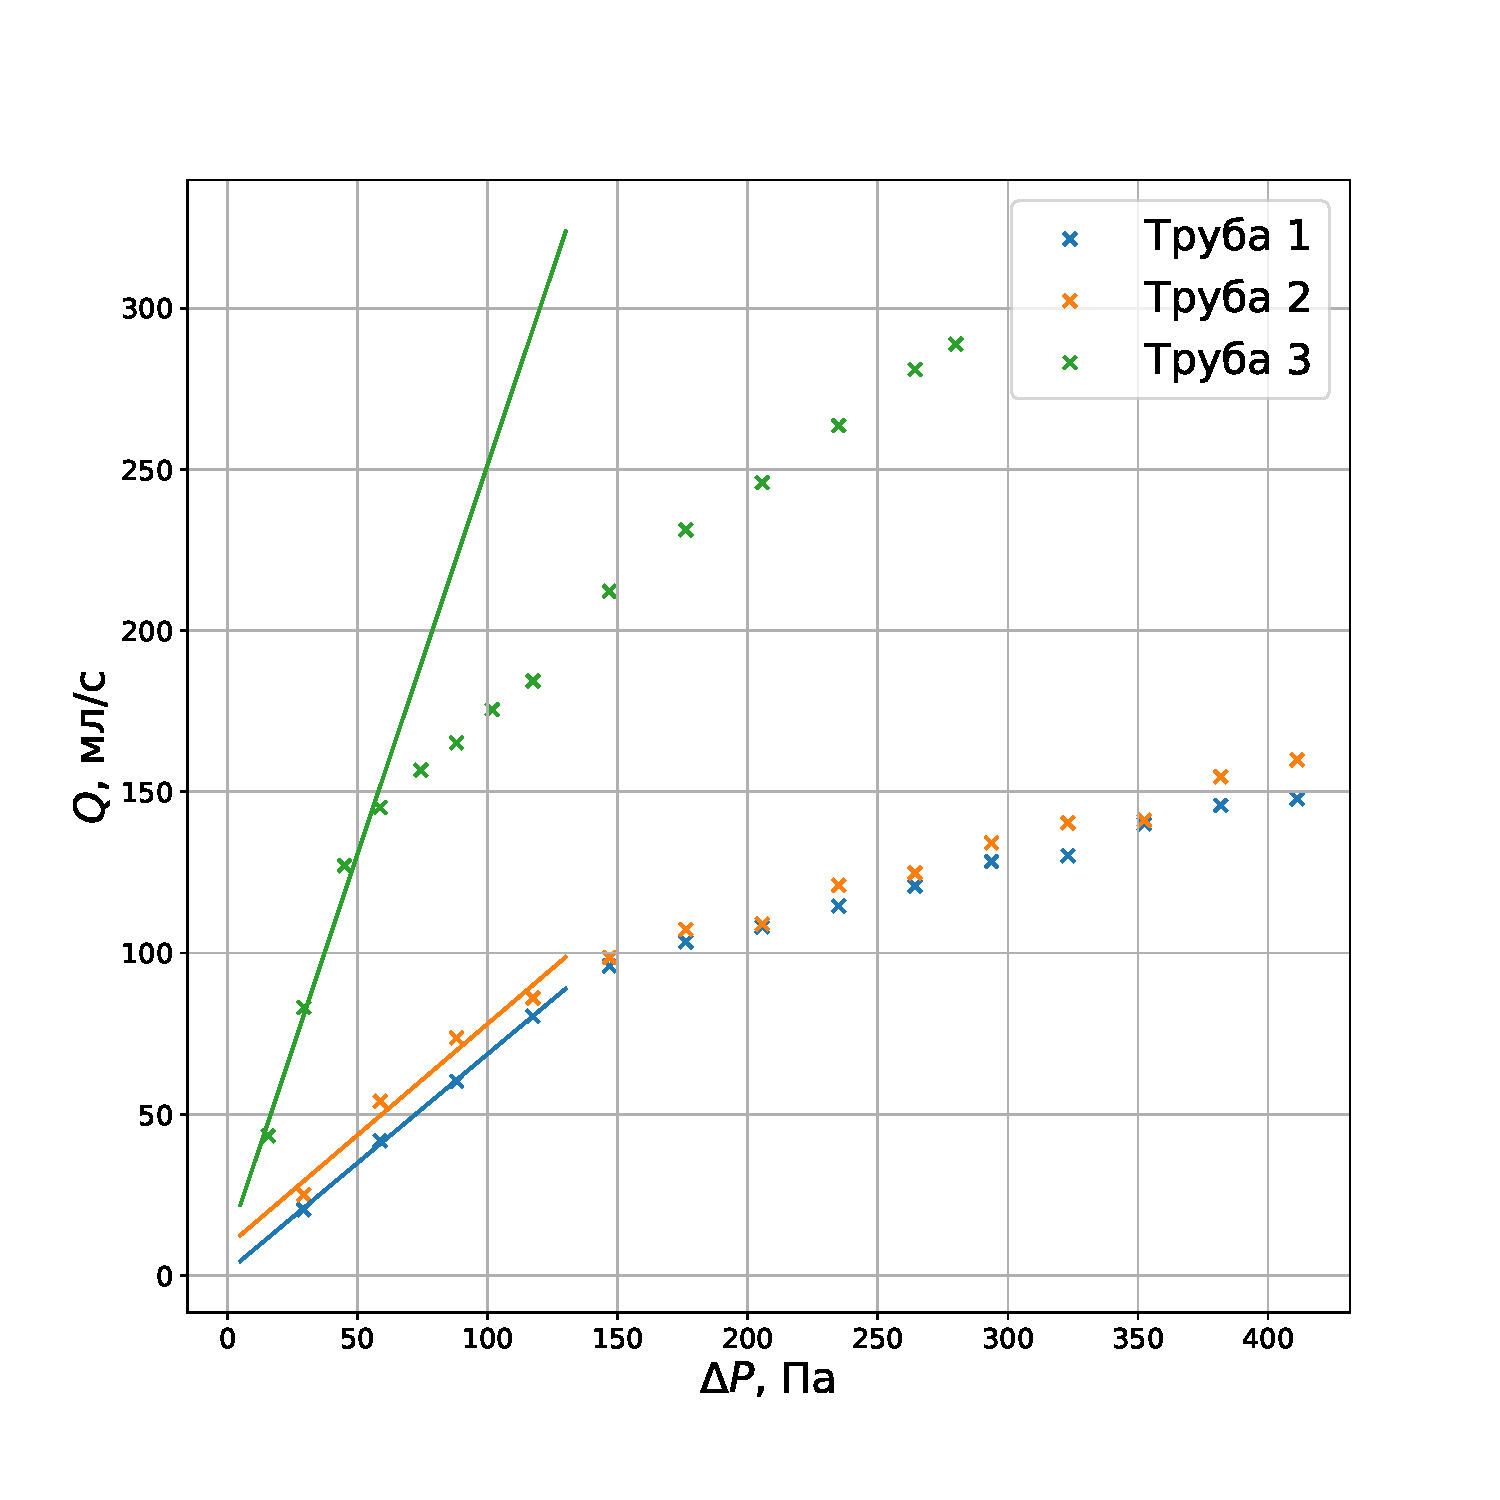
\includegraphics[scale = 0.4]{QP.pdf}
\end{figure}

Из него видно, что у каждого графика первые 4 точки соответствуют ламинарному течению (это видно и по построенным прямым). Для труб 1 и 2 это приблизительно давление в $150$ Па, а для 3 --- $50$ Па.

Так как коэффициенты наклона для этих случаев равны:

\[
\begin{aligned}
    k_1 &= 0,68 ~\frac{мл}{с \cdot Па},&~ \eps &= 1,3\% \\
    k_2 &= 0,69 ~\frac{мл}{с \cdot Па},&~ \eps &=   9\% \\
    k_3 &= 2,4  ~\frac{мл}{с \cdot Па},&~ \eps &=   8\% \\
\end{aligned}    
\]

Соответственно, по формуле можно найти вязкость воздуха:

\[
    \eta = \frac{\pi R^4}{8kl}
\]

\[
\begin{aligned}
    \eta_1 &= 1,63 \cdot 10^{-5} Па \cdot с,&~ \eps &=  2\% \\
    \eta_2 &= 1,20 \cdot 10^{-5} Па \cdot с,&~ \eps &= 10\% \\
    \eta_3 &= 1,53 \cdot 10^{-5} Па \cdot с,&~ \eps &=  9\% \\
\end{aligned}    
\]

% Тут нихуя не сошлось. В 1 и 3 я поделил на 20, а втором - на 6. И я хуй знает, что тут не так.

\point Построим по данным таблицы \ref{Tab:5} зависимость $P(x)$.

\begin{figure}[!h]
    \centering
    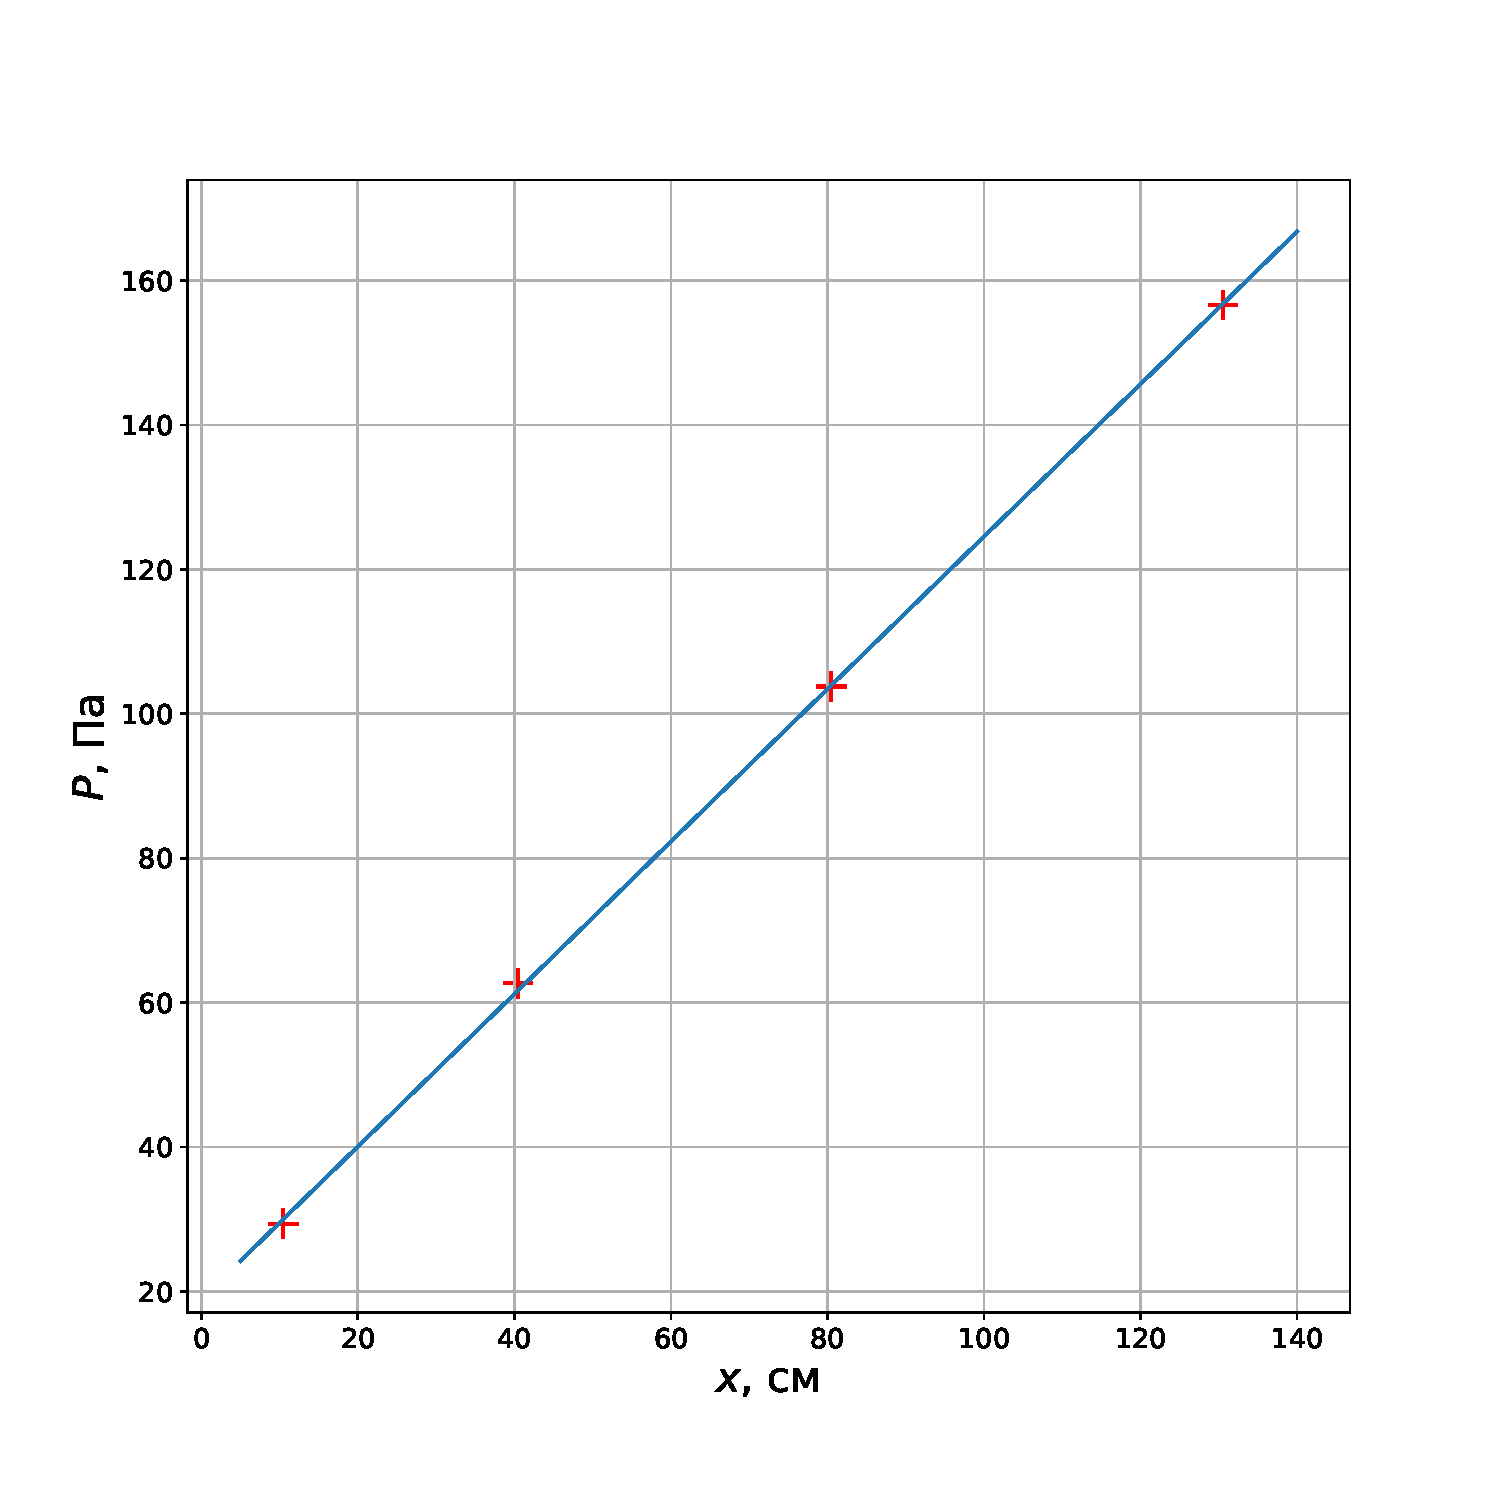
\includegraphics[scale = 0.4]{Px.pdf}
\end{figure}

Если присмотреться, то можно увидеть что первые две точки лежат не на прямой, а остальные - ровно на ней. Это означает, что ламинарный поток начинается приблизительно с $l_{уст} = 80$ см, что очень близко (2,4\%) к нашему прогнозу ($l_{уст} = 82$ cм).

\point Возьмём градиент $\displaystyle \frac{\Delta P}{l} = 1,96 ~\frac{Па}{см}$. Построим график $\ln Q (\ln R)$ для того, чтобы убедиться, что $Q \sim R^4$.

\begin{figure}[!h]
    \centering
    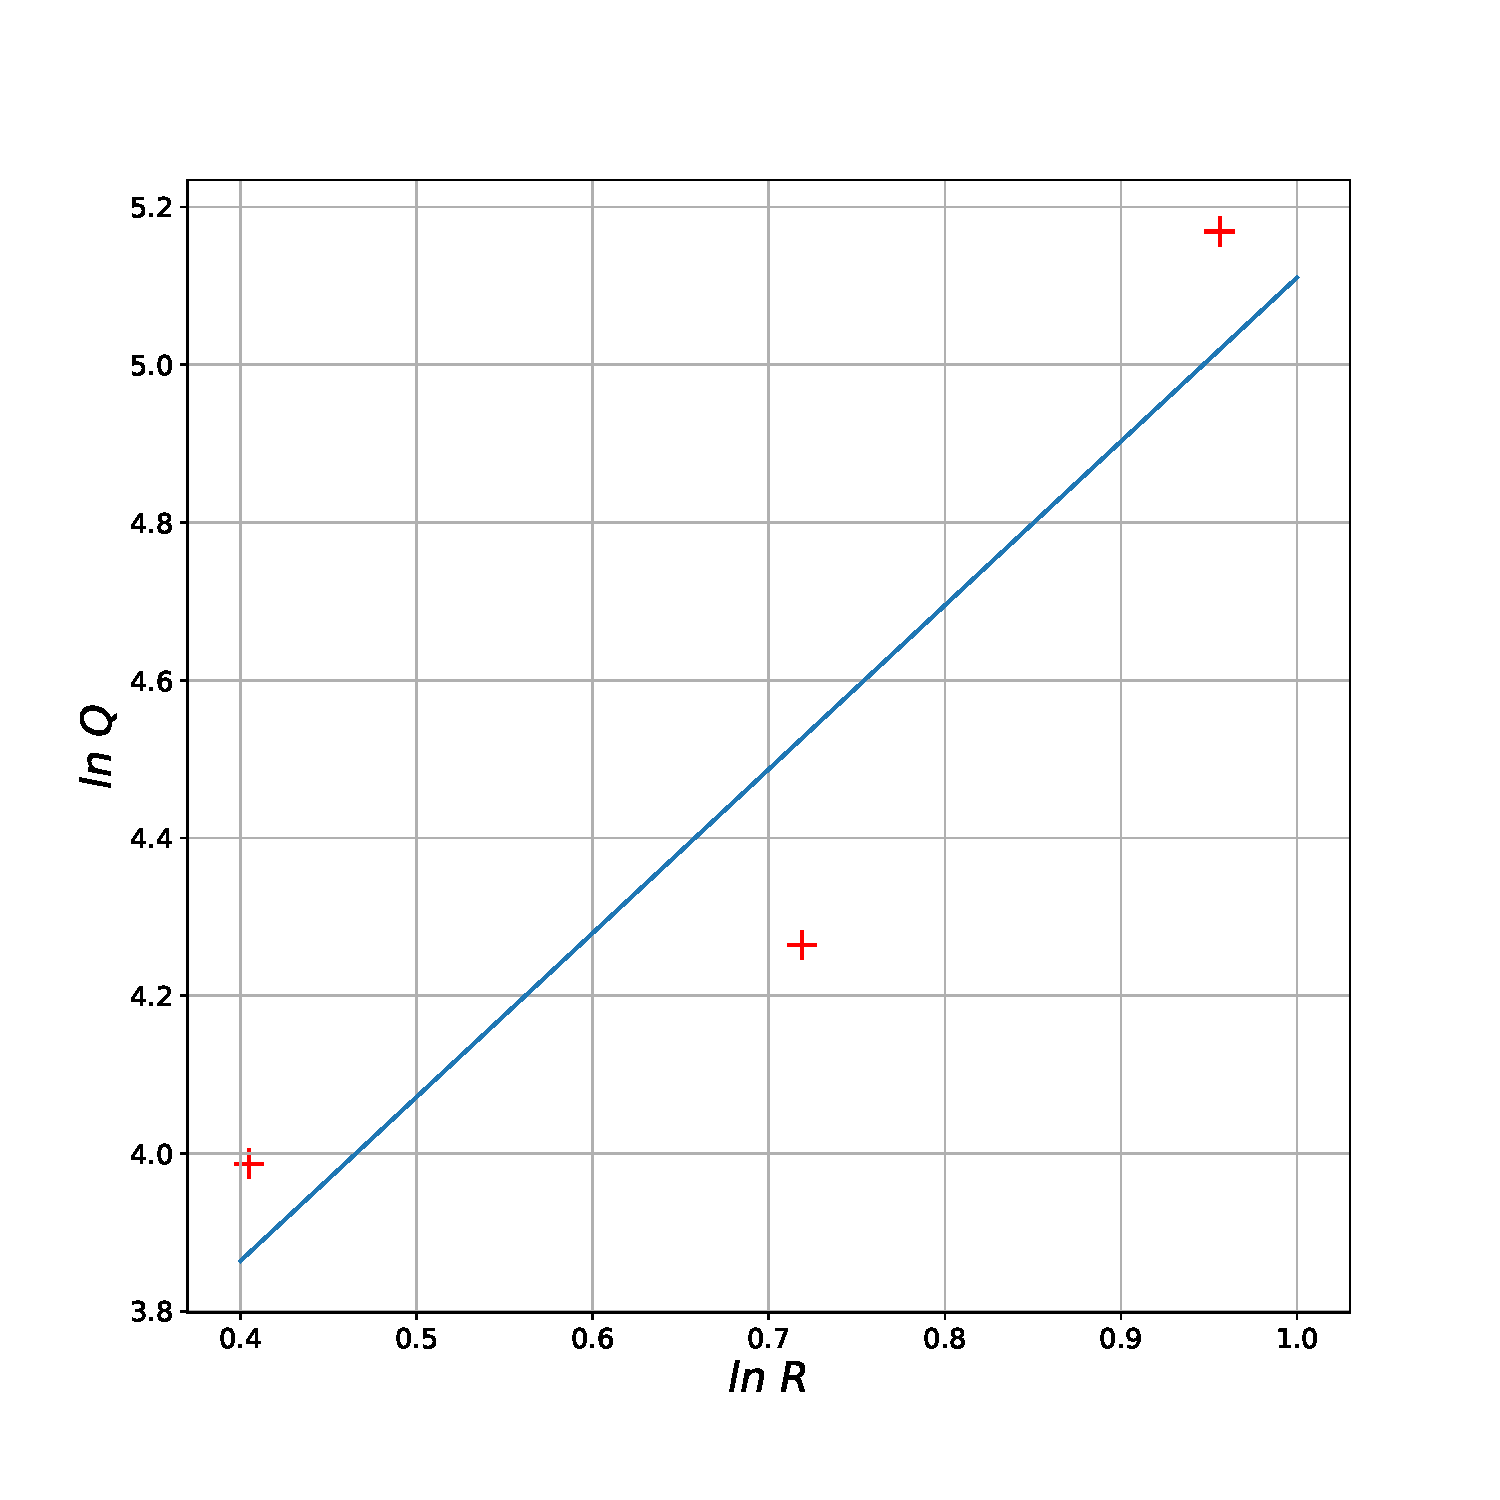
\includegraphics[scale = 0.4]{QR.pdf}
\end{figure}

Коэффициент наклона равен $k = 2,1 \pm 0,5$. К сожалению, это значение на $48\%$ отличается от ожидаемого $k = 4$. Скорее всего, такая ошибка связана с тем, что измерения проводились на турбулентном потоке, для которого $k = 2,5$. Здесь уже ошибка составляет всего $16\%$, что косвенно подтверждает наш тезис.

\end {document}
